\section{Preliminaries}
\label{sec:preliminaries}
In order to make the paper self-contained, we first introduce several preliminaries proposed in the unsupervised learning pipelines \cite{zhou2017unsupervised,}. The core idea behind, as discussed in \ref{sec:related}, is inverse warping from target view to source view with awareness of 3D geometry, as illustrated in Fig. \ref{fig:3d_warping}(a), which we will elaborate in the following paragraphs.

\paragraph{Perspective projection between multiple views.}
Let $D(x_t)$ be the depth value of the target view at image coordinate $x_t$, and $\ve{K}$ be the intrinsic parameter of the camera. Suppose the relative pose from the target view to source view is a rigid transformation $\ve{T}_{t\rightarrow s} = \{\ve{R} | \ve{t}\} \in \hua{S}\hua{E}(3)$, and $h(x)$ is the homogeneous coordinate given $x$. The perspective warping to localize corresponding pixels can be formulated as, 
\begin{align}
\label{eqn:warp}
D(x_s)h(x_s) = \ve{K}\ve{T}_{t\rightarrow s}D(x_t)\ve{K}^{-1}h(x_t),
\end{align}
and the image coordinate $x_s$ can be obtained by dehomogenisation of $d(x_s)h(x_s)$. Thus, $x_s$ and $x_t$ is a pair of matching coordinates, and we are able to compare the similarity between the two to valide the correctness of geometry.


\paragraph{Photometric error from view synthesis.} 
\label{chap:warping}
%that the color of each pixel is necessarily be similar after perspective projection for a static rigid scene
Given pixel matching pairs between target and source view, \ie $I_t$ and $I_s$, we can synthesis a target view $\hat{I_s}$ from the given source view through bilinear interpolation~\cite{GargBR16}, as illustrated in Fig. \ref{fig:3d_warping}(b). 
Then, under the assumption of Lambertian and a static rigid scene, average photometric error is often used to recover the depth map $D$ for the target view and the relative pose, \eg \cite{zhou2017unsupervised}. 
However, as pointed out by \cite{zhou2017unsupervised}, this assumption is not always true, due to the fact of existing moving object and occlusion. Thus, an explainability mask $\ve{M}$ is induced to leverage the issue. Formally, the masked photometric error is,

\begin{align}
\label{eqn:warp}
&\scr{E}_{vs}(D, \hua{T}, \hua{M}) = \sum_{s=1}^{S}\sum_{x_t}\ve{M}_s(x_t)|I_t(x_t) - \hat{I_s}(x_t)|, \nonumber \\
&\text{s.t. ~~} d(x) > 0, \any \ve{M}_s(x)\in [0, 1],
\end{align}
where $\{I_s\}_{s=1}^{S}$ is the set of source views, and $\hua{T}$ is a set of transformation from target view to each of the source views. 
$\hua{M} = \{\ve{M}_s\}$ is a set of explainability masks, and $\ve{M}_s(x_t) \in [0, 1]$ weights the error at $x_t$ from source view $s$.

%One main supervision of our framework comes from novel view synthesis: given an input view of a scene and camera motion, synthesize an image of the scene seen from a different view. 
% We can synthesize an image of the target view given the image of source view, camera motion from target view to source view and depth map of target view, using 3D inverse warping. The process of warping is shown in Figure \ref{fig:3d_warping}. 
\begin{figure}
\centering
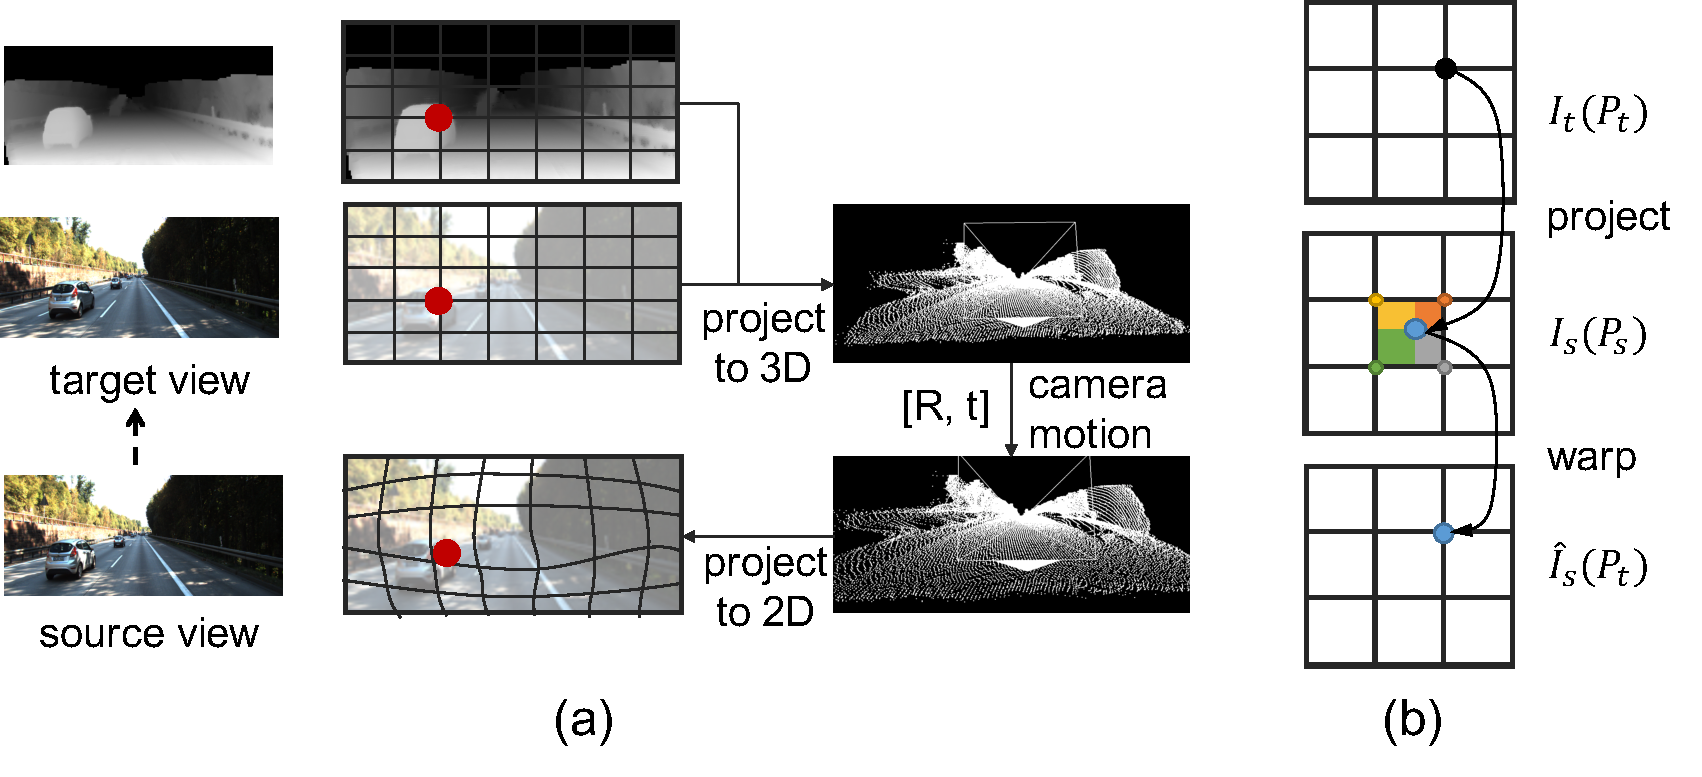
\includegraphics[width=0.5\textwidth]{figures/3d_warping.pdf}
\caption{Illustraion of (a) 3D inverse warping and (b) bilinear interpolation.}
\label{fig:3d_warping}
\end{figure}
% Each pixel (point on the grid) of depth map is first mapped onto 3D space. The 3D point cloud is transformed based on camera motion and then mapped back to 2D plane. Each grid point in target view corresponds to one point in source view. Similar to \cite{jaderberg2015spatial}, the bilinear interpolation is implemented to calculate each pixel value of warped image as a weighted sum of four nearest neighboring pixels in source image, weighted by the square area between the projected point and neighboring point, as shown in Figure \ref{fig:3d_warping} (b).

% The warping loss is a photometric difference between the target image and warped image. $$$$
% In which, $s$ iterates the number of source image, $p$ iterates each pixel in the image, $I_t$ is the target image, $I_s$ is the source image, $\hat{I_s} = \tau(I_s, D_t, Rt)$ is the warped image, $\tau$ is the warping function as introduced above.

\paragraph{Regularization.} 
As mentioned in \secref{sec:intro}, supervision based solely photometric error is ambiguous. One pixel could match to multiple candidates, especially at low-texture regions. In addition, there is trivial solution for explainability mask by setting all value to zero. Thus, to reduce depth ambiguity and encourage non-zero of masks, two regularization terms are applied, 
% One issue with using only view synthesis as supervision is that the back-propagation gradients are solely derived from the pixel value difference between one point in target image and weighted sum of its four neighboring points in source image. The warping loss will not be useful for learning where the point falls on low-texture regions. The predicted depth on these regions can be of any value as long as the warped region has the similar pixel value.  To overcome this issue, a prior knowledge of the scene geometry is incorporated for a smoothness loss:
\begin{align}
\small
\label{eqn:regular}
\scr{E}_{s}(D, 2) &= \sum_{x_t}\sum_{d \in {x, y}}|\nabla^{2}_dD(x_t)|e^{-\alpha|\nabla_dI(x_t)|} & \nonumber \\
\scr{E}_{m}(\hua{M}) &= -\sum_s\sum_{x_t}\log P(M_s(x_t) = 1) &
\end{align}
$\scr{E}_{s}(D, 2)$ is a spatial smoothness term penalizes L1 norm of second-order gradients of depth along both x and y direction, encouraging depth value align in planar surface when no image gradient appears. Here, the number $2$ represents the order of gradient \wrt the input.
 % As depth discontinuity often happens at image gradients, the smoothness loss is weighted by the a function of image gradients to prevent smoothed depth at image gradients. 

Finally, multi-scale strategy is applied to the depth output, and the total loss for depth estimation from video is a joint functional from previous terms,
\begin{align}
\small
\label{eqn:full}
\scr{E}_{o}(\{D_l\}, \hua{T}, \hua{M}) =& \sum_l\{\scr{E}_{vs}(D_l,\hua{T},\hua{M}) + \lambda_s\scr{E}_{s}(D_l) \nonumber\\
&+ \lambda_m\scr{E}_{m}(\hua{M}_l)\}
\end{align}

Given the objective function, the photometric error can be back-propagated to depth, pose and mask networks by applying the spatial transform operation as proposed by~\cite{jaderberg2015spatial}, which supervises the learning process.

